\chapter{Pollard-rho para resolver ECDLP}
Em 1978, Pollard veio com o método Monte-Carlo\footnote{Monte-Carlo é um método estatístico que se baseiam em amostragens aleatórias massivas para obter resultados numéricos, isto é, repetindo sucessivas simulações um elevado número de vezes, para calcular probabilidades de forma heurística.} para resolver o problema do logaritmo discreto. Desde então, o método foi modificado para resolver o ECDLP. Como o algoritmo Pollard-rho é atualmente o algoritmo mais rápido para resolver o ECDLP, então a segurança do ECC depende da eficiência desse algoritmo. Teoricamente, se o algoritmo Pollard-rho é capaz de resolver o ECDLP eficientemente e em um tempo relativamente curto, então o criptossistema estará inseguro. \cite{Mandy:2007}

A estratégia do algoritmo é produzir uma sequência de termos gerados randomicamente $(a_k, b_k, R_k)$, onde \(R_k\) é um ponto na curva \(E\) e \(a_k\)  e \(b_k\) estão em $\mathbb{F}_p$ sobre a qual a curva elíptica \(E\) está definida. Como $E(\mathbb{F}_p)$ é um grupo finito, a sequência eventualmente irá torna-se periódica e voltará para um termo anterior da sequência \--- tal ocorrência é chamada de \textit{colisão}. Usa-se essa periodicidade para resolver ECDLP. Como nem sempre a sequência volta para o primeiro termo, um diagrama da sequência parecerá com a letra Grega \(\rho\) (Ver figura \ref{fig:rho}). Por este motivo esse método é chamado de Pollard-rho. Essa sequência de termos gerados é chamada de ``percurso''.

Seja \(\mu\) o tamanho da calda e \(\lambda\) o tamanho do ciclo. Após um número finito de iterações, obtêm-se os termos $R_k = R_{k+\lambda}$, onde $k > \mu$ e $\lambda > 1$. Neste ponto, já deverá ter sido encontrado uma correspondência entre os termos e poderá aplicar matemáticas discretas para resolver os problemas de logaritmo discreto gerado pelos elementos do conjunto finito.

A seguir serão apresentados o algoritmo de Pollard-rho e suas variações.

\begin{figure}[h]
\centering
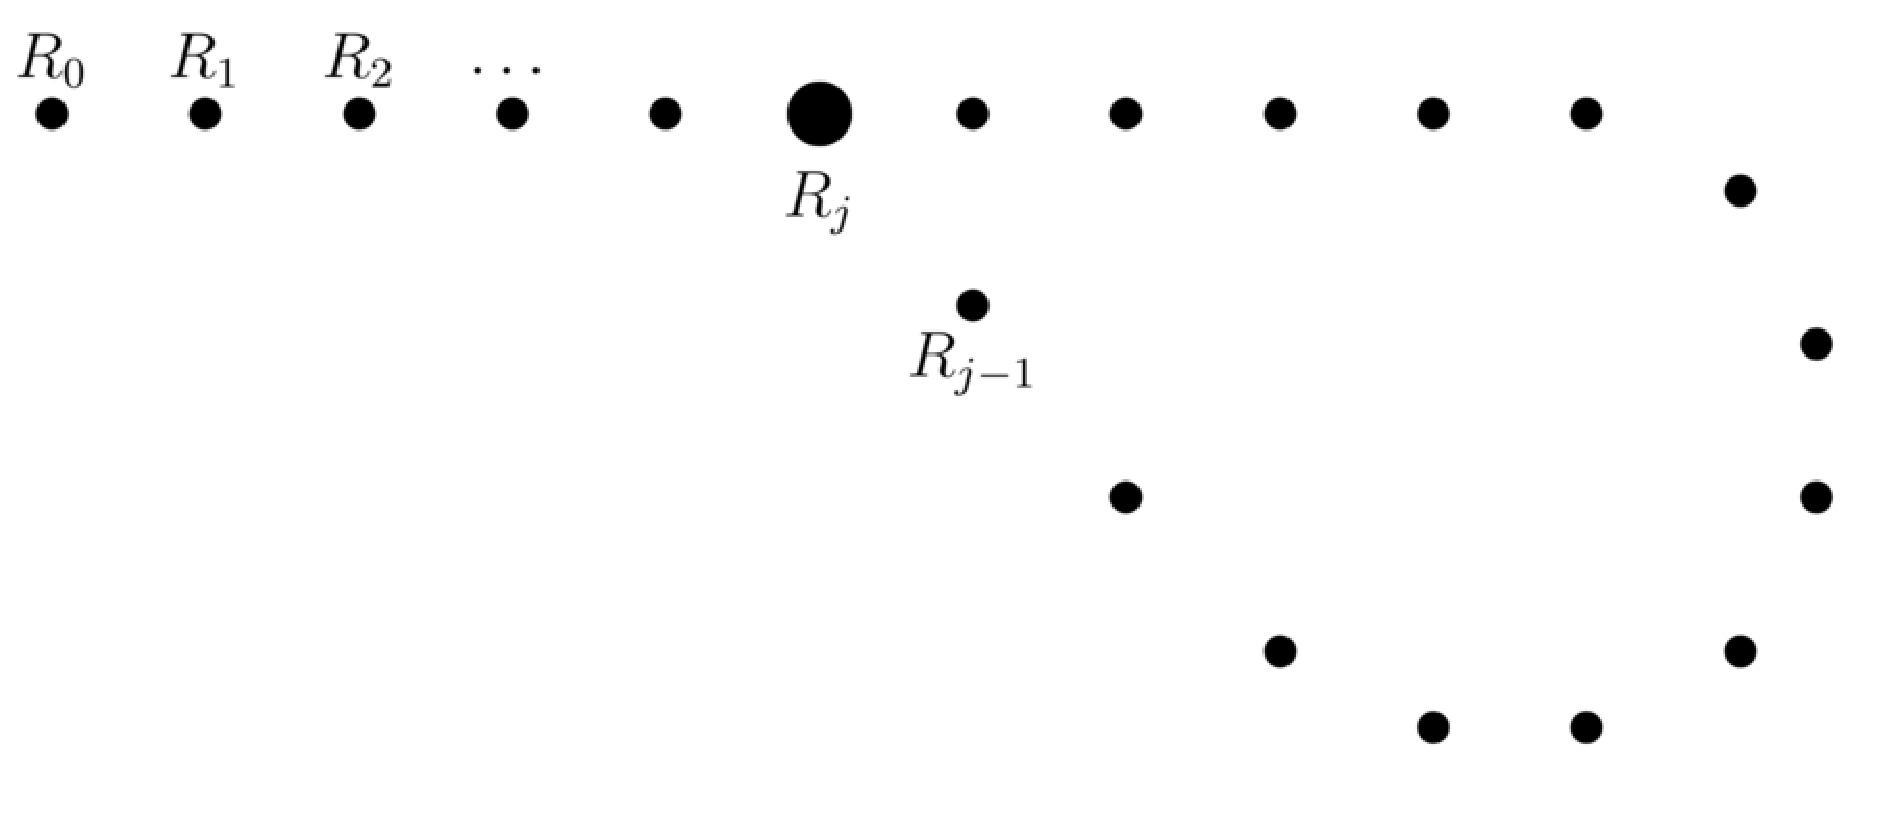
\includegraphics[scale=0.4, bb=0 0 888 376]{figuras/rho.eps}
\caption{Diagrama da sequência produzida pelo algoritmo Pollard-rho}
\label{fig:rho}
\end{figure}

\section{Pollard-rho original}
Seja $G = E(\mathbb{F}_p)$, tal que a ordem de $G = n$, e \(P\) e \(Q\) tal que $Q = xP$ em \(G\). O objetivo é calcular \(x\). Segue os passos:

\begin{enumerate}
\item \(G\) é particionado em 3 conjuntos $S_1, S_2, S_3$ de aproximadamente do mesmo tamanho, em que $\mathcal{O} \notin S_2$.
\item Definir uma função de iteração $f : R \to R$ de um percurso aleatório:

\begin{eqnarray} \label{eq:walk}
R_{k+1} = f(R_k) =
\begin{cases}
Q + R_k, &R_k \in S_1 \\
2R_k, &R_k \in S_2 \\
P + R_k, &R_k \in S_3
\end{cases}
\end{eqnarray}

\item Seja $R_k = a_kP + b_kQ$, e portanto

\begin{eqnarray}
a_{k+1} =
\begin{cases}
a_k, &R_k \in S_1 \\
2a_k \pmod n, &R_k \in S_2 \\
a_k + 1, &R_k \in S_3
\end{cases}
\end{eqnarray}

e

\begin{eqnarray}
b_{k+1} =
\begin{cases}
b_k + 1, &R_k \in S_1 \\
2b_k \pmod n, &R_k \in S_2 \\
b_k, &R_k \in S_3
\end{cases}
\end{eqnarray}

\item Os termos iniciais são: $R_0 = P, a_0 = 1, b_0 = 0$ e os pares gerados $(R_k, R_{2k})$ até encontrar uma correspondência $R_m = R_{2m}$, para qualquer \(m\).

\item Uma vez encontrados, calcule:

\begin{eqnarray*}
R_m = a_mP + b_mQ \\
R_{2_m} = a_{2_m}P + b_{2m}Q
\end{eqnarray*}

\item Com isso, é possível calcular \(x\):

\begin{equation} \label{eq:x}
x = (a_{2m} - a_m)(b_m - b_{2m})^{-1} \pmod n
\end{equation}

\end{enumerate}

O termo $(b_m - b_{2m})^{-1}$ em \ref{eq:x} somente é possível calcular quando o GCD$(b_m - b_{2m}, n) = 1$, ou seja, quando \(b_m\) e \(b_{2m}\) são coprimos entre si. Caso contrário, o algoritmo não poderá continuar.

%
% Pollar-rho com um processador
%
\section{Pollard-rho com único processador}
O método original seleciona inteiros aleatórios $a, b \in [0, n-1]$ e armazena as triplas $(a, b, aP + bQ)$ em uma tabela ordenada pelo terceiro componente até que um ponto $aP + bQ$ seja obtida pela segunda vez. Pelo paradoxo do aniversário
\footnote{Suponha que uma urna tenha \(n\) bolas numeradas de 1 a \(n\). As bolas são aleatoriamente retiradas uma de cada vez e colocadas de volta na urna. Portanto, o número esperado para que as bolas se repitam é de aproximadamente de $\sqrt{\pi n/2}$. Se \(n\) = 365 e as bolas representam diferentes dias do ano, então pode-se dizer que o número esperado de pessoas que tem de ser reunidas em uma sala para que pelo menos duas delas tenham nascido no mesmo dia é de aproximadamente $\sqrt{\pi 365/2} \approx 24$. Esse número é surpreendentemente pequeno e, consequentemente, daí vem a nomenclatura ``paradoxo do aniversário''. \cite{Guide}},
o número de iterações esperado até que se obtenha uma colisão é de aproximadamente $\sqrt{\pi n/2} \approx 1.2533 \sqrt{n}$. A desvantagem desse algoritmo é que a capacidade de armazenamento necessária para o cálculo é de $\sqrt{\pi n/2}$ triplas.

A modificação desse algoritmo encontra os pares ($a_m, b_m$) e ($a_{2m}, b_{2m})$ aproximadamente no mesmo tempo que o método original, mas tem desprezíveis requisitos de armazenamento. A ideia é definir uma função de iteração $f : \langle P \rangle \to \langle P \rangle$ de modo que $X \in \langle P \rangle$ e $a, b \in [0, n-1]$ com $X = aP + bQ$. Além disso, \(f\) deve ter características de uma função aleatória.

Seja $\{S_1, S_2, ..., S_L\}$ uma partição aleatória de $\langle P \rangle$ em uma quantidade \(L\) de conjuntos de aproximadamente do mesmo tamanho. Então um ponto $X \in \langle P \rangle$ pode ser designado a \(S_j\) se os cinco \textit{bits} menos significantes da coordenada \(x\) de \(X\) representam o inteiro \(j-1\). Desta forma, define-se $j = H(X)$ se $X \in S_j$, no qual \(H\) é uma função de partição. Finalmente, seja $c_j, d_j \in [0, n-1]$ para $1 \leq j \leq L$. Então $f : \langle P \rangle \to  \langle P \rangle$ é definido por

\begin{equation*}
f(X) = X + c_jP + d_jQ \textrm{, onde } j = H(X)
\end{equation*}

\textit{O algoritmo recebe como parâmetro uma curva elíptica \(E\) e dois pontos \(P\) e \(Q\) pertencentes a \(E\) e calcula o valor de \(x\) tal que $x = \log_P Q$.}

% 
% INPUT: EllipticCurve E, Point P, Point Q
% OUTUPT: x = log_P(Q)
%
\begin{lstlisting}[caption={Algoritmo Pollard-rho com único processador.},label=single_processor]
pollardRho_singleProcessor(E: Curva, P: Ponto, Q: Ponto): inteiro
	seja L, k, inteiro
	seja an, bn, inteiro
	seja am, bm, inteiro
	seja Xn, Xm, Ponto
	seja c, d, array inteiro
	seja R, array Ponto

	k := E.order()
	para j := 1, enquanto j <= L, faca
		c[j] := random() % k
		d[j] := random() % k
		R[j] := c[j]*P + d[j]*Q

	an := random() % k
	bn := random() % k
	Xn := an*P + bn*Q
	am := an
	bm := bn
	Xm := Xn

	enquanto Xn != Xm faca
		j := H(Xn, L)
		Xn := Xn + R[j]
		an := an + c[j]
		bn := bn + b[j]

	se bn = bm entao
		retorne "falha"

	seja x, inteiro
	x := (an - am)/(bm - bn) % k
	retorne x

H(P: Ponto, L: inteiro): inteiro
	retorne P.x % L + 1

\end{lstlisting}

%
% Pollard-rho com multiprocessadores
%
\section{Pollard-rho multiprocessadores}
Suponha agora que \(M\) processadores estão disponíveis para resolver uma instância de ECDLP. Uma abordagem normal seria de executar o algoritmo Pollard-rho independente para cada processador (com diferentes pontos \(X_0\) aleatórios escolhidos inicialmente) até que algum dos processadores finalize. Uma análise cuidadosa mostra que o número esperado de operações de curva elíptica executadas por cada processador até que algum finalize é de $3\sqrt{n/M}$. Assim a aceleração esperada é dada pelo fator $\sqrt{M}$. \cite{Guide}

Van Oorschot e Wiener propuseram uma variante do algoritmo Pollard-rho que produz um fator de aceleração \(M\) quando \(M\) processadores são empregados. A ideia é permitir as sequências $\{X_i\}_{i \geq 0}$ geradas por um processador para colidir com outro. Ou seja, cada processador escolhe randomicamente seu próprio ponto inicial \(X_0\), mas todos processadores utilizam a mesma função de iteração \(f\) para calcular os pontos subsequentes \(X_i\). Desta forma, se a sequência de dois diferentes processadores sempre se colidem, então, como ilustrados na Figura \ref{fig:paralellized}, as duas sequências serão idênticas daquele ponto em diante. \cite{Van:1996}

\begin{figure}[h]
\centering
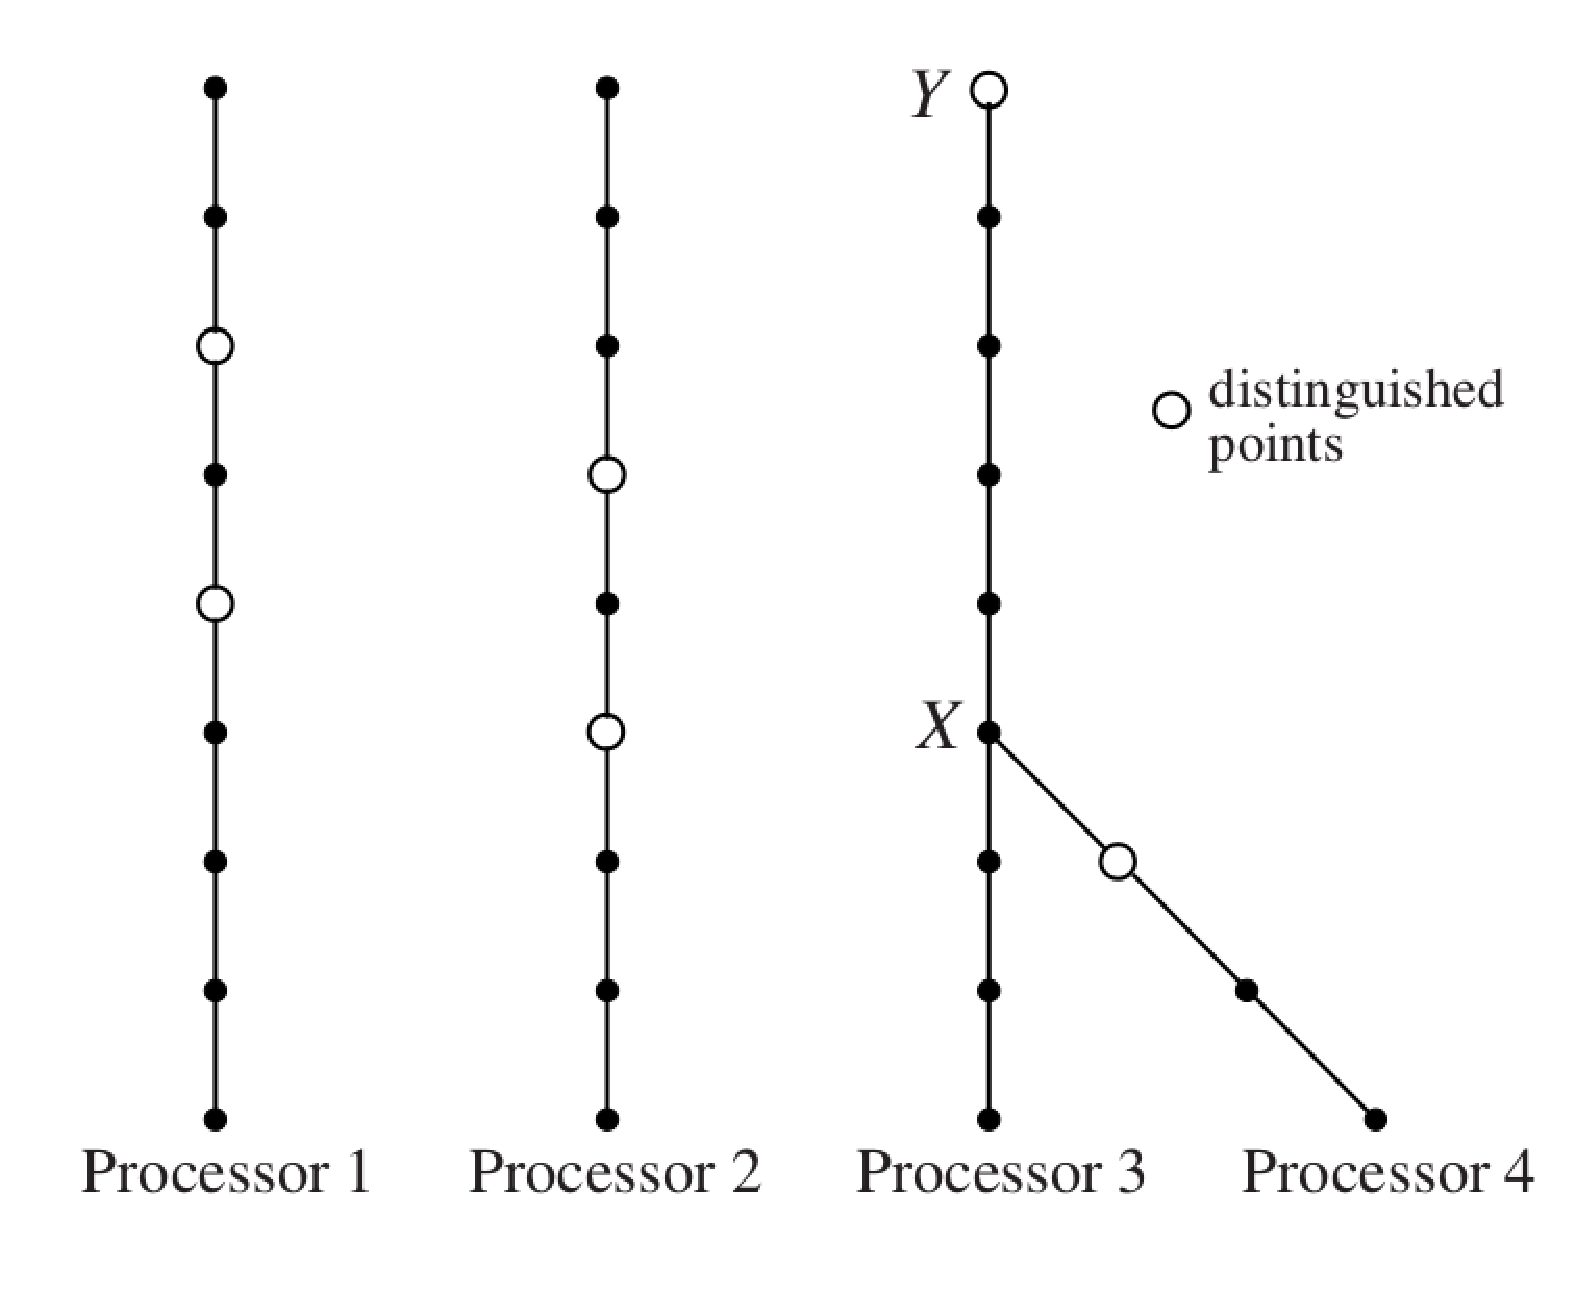
\includegraphics[scale=0.4, bb=0 0 737 604]{figuras/paralellized.eps}
\caption{A sequência gerada pelo algoritmo Pollard-rho paralelizado. A sequência gerada pelos processadores 3 e 4 se colidem em X. O algoritmo informa a coisão em Y, o primeiro ponto distinto subsequente.}
\label{fig:paralellized}
\end{figure}

O algoritmo apresentado na seção anterior encontra uma colisão na sequência gerada por um único processador. A seguinte estratégia possibilita uma procura eficiente de uma colisão nas sequências geradas por diferentes processadores. Uma \textit{propriedade distintiva} facilmente testável de pontos é selecionada. Por exemplo, um ponto deve ser \textit{distinto} se os primeiros \(t\) \textit{bits} de sua coordenada \(x\) são iguais a zero. Seja \(\theta\) a proporção em $\langle P \rangle$ tendo essa propriedade distintiva. Sempre que um processador encontra um ponto distinto, ele transmite o ponto a um servidor central que o armazena em uma lista ordenada. Quando o servidor recebe o mesmo ponto distinto pela segunda vez, ele calcula o logaritmo discreto desejado pela Equação \ref{eq:x} e termina a execução de todos os processadores. O número esperado de passos por processador antes de uma colisão ocorrer é de $(\sqrt{\pi n/2})/M$. Um ponto distinto subsequente é esperado para após $1/\theta$ passos. Consequentemente o número esperado de operações de curva elíptica desempenhadas por cada processador antes de uma colisão de pontos distintos é de

\begin{equation}
\dfrac{1}{M} \sqrt{\dfrac{\pi n}{2}} + \dfrac{1}{\theta}
\end{equation}

A sua versão paralelizada do algoritmo Pollard-rho obtém um aumento de velocidade que é linear em relação à quantidade de processadores empregados. Uma observação que deve ser feita é que os processadores não tem de comunicar-se entre si, e além disso tem uma comunicação limitada com o servidor central. Portanto, o espaço total necessário no servidor pode ser contolado com uma seleção cautelosa da propriedade distintiva.

\textit{O algoritmo recebe como parâmetro uma curva elíptica \(E\) e dois pontos \(P\) e \(Q\) pertencentes a \(E\) e calcula o valor de \(x\) tal que $x = \log_P Q$.}

%
% INPUT: EllipticCurve E, Point P, Point Q
% OUTUPT: x = log_P(Q)
%
\begin{lstlisting}[caption={Algoritmo Pollard-rho paralelizado.},label=parallelized]
pollardRho_parallelized(E: Curva, P: Ponto, Q: Ponto): inteiro
	seja L, k, inteiro
	seja an, bn, inteiro
	seja am, bm, inteiro
	seja Xn, Xm, Ponto
	seja c, d, array inteiro
	seja R, array Ponto

	seja a, b, inteiro
	seja X, ponto
	seja Y, Point

	k := E.order()
	para j := 1, enquanto j <= L, faca
		c[j] := random() % k
		d[j] := random() % k
		R[j] := c[j]*P + d[j]*Q

	# para cada processador M faca
	a := random() % k
	b := random() % k
	X := an*P + bn*Q

	# repita ate que o servidor receba um ponto Y distinto pela 2a vez
	enquanto duplicatedDistinguishedPointNotReceived() faca
		se X = distinguishedPoint(X)
			sendToServer(a, b, X)
			j := H(X)
			X := X + R[j]
			a := a + c[j] % k
			b := b + d[j] % k

	an := firstTripleCollided_a()
	bn := firstTripleCollided_b()
	am := secondTripleCollided_a()
	bm := secondTripleCollided_b()

	se bn = bm entao
		retorne "falha"

	seja x, inteiro
	x := (an - am)/(bm - bn) % k
	retorne x

H(P: Ponto, L: inteiro): inteiro
	retorne P.x % L + 1

\end{lstlisting}

%
% Pollard-rho com automorfismo
%
\section{Pollard-rho com automorfismo}

Uma maneira descrita por Hankerson, Menezes e Vanstone para acelerar o algoritmo Pollard-rho é fazendo uso de automorfismo.\cite{Guide}

Seja o grupo de pontos da curva elíptica $E(\mathbb{F}_q)$. Considere o ponto P de ordem \(n\) e o subgrupo gerado por esse ponto, ou seja, $\langle P \rangle$. Seja o automorfismo $\psi: \langle P \rangle \to \langle P \rangle$. A ordem da função $\psi$ é o menor inteiro positivo $t$ tal que $\psi^t(R) = R$ para todo ponto $R \in \langle P \rangle$.

É possível definir uma relação de equivalência $R_1 \sim R_2$ se e somente se $R_1 = \psi^j(R_2)$ para algum $j \in [0, t - 1]$. Daí cria-se a classe de equivalência $[R]$, que é descrita por
$$
[R] = \{R, \psi(R), \psi^2(R), \dots, \psi^{l-1}(R)\}
$$
onde $l$ é o menor divisor positivo da ordem $t$ da função $\psi$, tal que $\psi^l(R) = R$.

O método de Pollard Rho com automorfismo consiste em utilizar uma função iterativa $f$ que seja definida nas classes de equivalência. Para isso, será definido um representante $\overline{R}$ para a classe de equivalência $[R]$ e uma função $g$ tal que
$$
g(R) = \overline{f(R)}
$$

Sendo conhecido um inteiro $\lambda \in [0, n - 1]$ tal que $\psi(P) = \lambda P$ e os inteiros $a,b$ tal que $X = aP + bQ$, então pode-se calcular $\overline{X} = \overline{a}P + \overline{b}Q$ eficientemente por $\overline{a} = \lambda^{j}a \mbox{mod \textit{n}}$ e $\overline{b} = \lambda^{j}b \mbox{mod \textit{n}}$.
